\documentclass[12pt, twoside]{article}
\usepackage[francais]{babel}
\usepackage[T1]{fontenc}
\usepackage[latin1]{inputenc}
\usepackage[left=5mm, right=5mm, top=5mm, bottom=5mm]{geometry}
\usepackage{float}
\usepackage{graphicx}
\usepackage{array}
\usepackage{multirow}
\usepackage{amsmath,amssymb,mathrsfs}
\usepackage{soul}
\usepackage{textcomp}
\usepackage{eurosym}
 \usepackage{variations}
\usepackage{tabvar}
\usepackage{lscape}


\pagestyle{empty}

\begin{document}




\section*{\center{Correction devoir maison 7}}

\subsection*{Exercice 1}

Odile  s'est tromp�e:  $1 \div 3  \neq 0,33$  car $0,33 \times 3 =0,99$.
\qquad \qquad Laurent a raison car $0,8 \times 5=4$.

Abdou a tort: $1 \div 8 =0,125 \neq 1,12$. \qquad \qquad 
Th�o a tort: $3 \times 1,67 =5,01 \neq 5$.

\subsection*{Exercice 2}

$\dfrac{2}{3}=\dfrac{6}{9}$ \qquad \quad $\dfrac{2}{3}=\dfrac{12}{18}$ \qquad
\quad  $\dfrac{2}{3}=\dfrac{10}{15}$
\qquad \quad $\dfrac{3}{4}=\dfrac{21}{28}$ \qquad
\quad $\dfrac{3}{4}=\dfrac{21}{28}$
\qquad \quad $\dfrac{5}{6}=\dfrac{15}{18}$ \qquad \quad
$\dfrac{5}{6}=\dfrac{10}{12}$ \qquad \quad $\dfrac{5}{6}=\dfrac{20}{24}$


\subsection*{Exercice 3}

La descente correspond � $\dfrac{4}{7}$ du trajet total.
La rivi�re correspond � $\dfrac{1}{7}$ du trajet total.


\subsection*{Exercice 4}

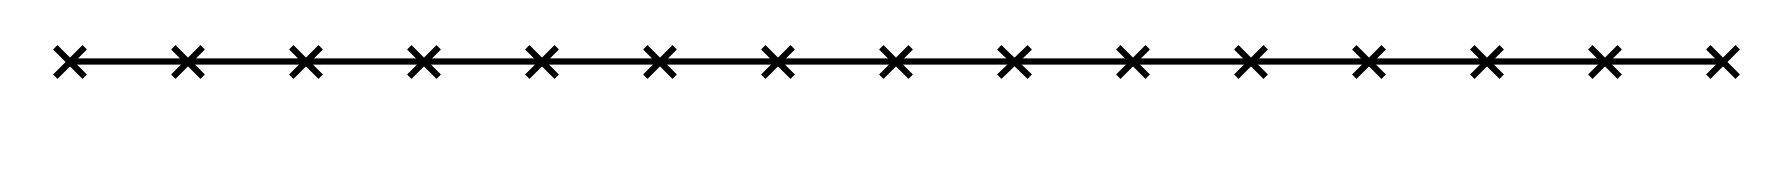
\includegraphics[width=9cm]{images/ex4.png} 


\subsection*{Exercice 5}


\begin{enumerate}
\item $\dfrac{1}{6} \times 30=\dfrac{30}{6}=5$ \qquad \qquad $\dfrac{3}{10}
\times 30=\dfrac{90}{10}=9$ \qquad \qquad $\dfrac{2}{5} \times 30=\dfrac{60}{5}=12$

\enskip

Dans le verre de 30 cl, il ya 5 cl de jus d'orange, 9 cl de jus de raisin et 12
cl de jus de pomme.


\item 30 - 5 - 12 - 9 = 4 \quad Il y a 4 cl de jus de mangue.

\item En vert: 10 carreaux � colorier, en rouge: 18 carreaux � colorier, en
bleu: 24 carreaux � colorier.

\item Il reste 8 carreaux non colori�s, il y en a 60 au total donc la fraction
est $\dfrac{8}{60}$.

\item $\dfrac{8}{60} \times 30= \dfrac{240}{60}=4$. On retrouve les 4 cl
calcul�s pr�cedemment.
\end{enumerate}


\subsection*{Exercice 6}


Horizontalement:

\enskip

I. $\dfrac{1}{4} \times \ldots = 148$ donc le nombre � trouver est 592 ($148
\times 4 = 592$).

\enskip

II. $\dfrac{2}{3} \times 18 = 2 \times 6 = 12$ \qquad \qquad
III. $\dfrac{19}{5}=\dfrac{152}{40}$

\enskip

IV. A partir du 3, on trouve le nombre 36 (car 6 est le double de 3).

\enskip


Verticalement:

\enskip

1. A partir du II et III, on trouve le nombre 111 (tous ces chiffres sont
�gaux).
\qquad  \qquad 2. $\dfrac{5}{21}=\dfrac{125}{525}$

\enskip

3. $\dfrac{93}{4}=23,25$ et $\dfrac{1}{4}=0,25$. \qquad  $\dfrac{93}{4}= \ldots
+ \dfrac{1}{4}$ donc $23,25= \ldots + 0,25$. Le nombre manquant est 23.

\enskip

4. A partir du I, on cherche un nombre divisible par 9 dont la dizaine est 2:
c'est 27.
\end{document}
